\documentclass[a4paper, 12pt, twocolumn]{article}
\usepackage{graphicx}  
\usepackage{wrapfig}
\usepackage[brazilian]{babel}
\usepackage{amsmath}
\usepackage{hyperref}
\usepackage[utf8]{inputenc}
\usepackage{cuted}
\usepackage{amsfonts}
\usepackage{listings}
\usepackage{siunitx}

\lstset{literate=
  {á}{{\'a}}1 {é}{{\'e}}1 {í}{{\'i}}1 {ó}{{\'o}}1 {ú}{{\'u}}1
  {Á}{{\'A}}1 {É}{{\'E}}1 {Í}{{\'I}}1 {Ó}{{\'O}}1 {Ú}{{\'U}}1
  {à}{{\`a}}1 {è}{{\`e}}1 {ì}{{\`i}}1 {ò}{{\`o}}1 {ù}{{\`u}}1
  {À}{{\`A}}1 {È}{{\'E}}1 {Ì}{{\`I}}1 {Ò}{{\`O}}1 {Ù}{{\`U}}1
  {ä}{{\"a}}1 {ë}{{\"e}}1 {ï}{{\"i}}1 {ö}{{\"o}}1 {ü}{{\"u}}1
  {Ä}{{\"A}}1 {Ë}{{\"E}}1 {Ï}{{\"I}}1 {Ö}{{\"O}}1 {Ü}{{\"U}}1
  {â}{{\^a}}1 {ê}{{\^e}}1 {î}{{\^i}}1 {ô}{{\^o}}1 {û}{{\^u}}1
  {Â}{{\^A}}1 {Ê}{{\^E}}1 {Î}{{\^I}}1 {Ô}{{\^O}}1 {Û}{{\^U}}1
  {œ}{{\oe}}1 {Œ}{{\OE}}1 {æ}{{\ae}}1 {Æ}{{\AE}}1 {ß}{{\ss}}1
  {ű}{{\H{u}}}1 {Ű}{{\H{U}}}1 {ő}{{\H{o}}}1 {Ő}{{\H{O}}}1
  {ç}{{\c c}}1 {Ç}{{\c C}}1 {ø}{{\o}}1 {å}{{\r a}}1 {Å}{{\r A}}1
  {€}{{\euro}}1 {£}{{\pounds}}1 {«}{{\guillemotleft}}1
  {»}{{\guillemotright}}1 {ñ}{{\~n}}1 {Ñ}{{\~N}}1 {¿}{{?`}}1
  {ã}{{\H{a}}}1
}

\linespread{1.0}

\title{Analogias clássicas para helimagnetos}
\author{Danilo Lessa Bernardineli}
\date{03.~Novembro 2017}

\begin{document}

%%%%%%
\begin{strip}
\maketitle

%%
\abstract{Neste trabalho, é feita a elaboração de dois modelos magnetostáticos em um cilindro na qual a magnetização oscila ao longo da altura do mesmo. É feita a caracterização das correntes superficiais e volumétricas ligadas e notou-se o surgimento de duplas de vórtices/anti-vórtices em um deles. A inspiração do trabalho é em fazer uma analogia clássica aos helimagnetos.}
\end{strip}

%%%%%%
\section{Introdução}

\subsection{O que é um Helimagneto?}

Helimagnetos são magnetos caracterizados por uma magnetização helicoidal a qual pode ser visualizada como sendo ferromagnetos com magnetização orientadas em uma direção ligeiramente diferente em cada plano sucessivo. Uma ilustração dele pode ser vista na figura \ref{fig:helimagneto}.

A origem do ordenamento helimagnético em um material, de acordo com o modelo de Heisenberg,  vem da competição entre interações de troca que dão origem ao ordenamento ferromagnético e antiferromagnetico - deste modo, tanto o ferromagnetismo quanto o antiferromagnetismo podem ser enxergados como casos particulares do helimagnetismo mediante um ângulo característico tendendo a zero ou a \ang{180} respectivamente. \cite{lecture_29}\cite{helimagnetism-heisenberg-model}

\begin{figure*}
    \caption{Ilustração da magnetização de um helimagneto. A flecha representa a magnetização do material, e $a$ seria um parâmetro de rede.\protect\footnote{https://encyclopedia2.thefreedictionary.com/Magnetic+Structure} }
    \centering
    \label{fig:helimagneto}
    \vspace{0pt}
    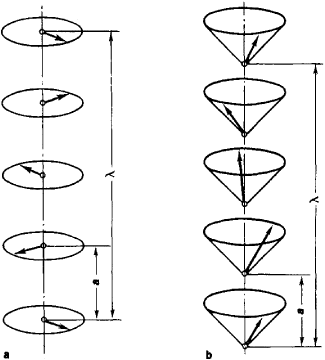
\includegraphics[width=0.5\textwidth]{heli.png}
\end{figure*}

\subsection{Objetivos do trabalho}

A proposta deste trabalho é de explorar modelos magnetostáticos que façam uma analogia com os helimagnetos reais no sentido de existir uma variação do vetor magnetização ao longo do eixo de cilindro.

Serão explorados dois modelos neste trabalho:

\begin{itemize}
\item Cilindro com magnetização helicoidal em torno do eixo de simetria.
\item Cilindro com magnetização helicoidal perpendicular a base do cilindro.
\end{itemize}

O procedimento passará por levantar hipóteses nos modelos, fazer a caracterização das correntes ligadas associadas com a magnetização helicoidal e finalmente gerar visualizações destes.

%%%%%% %%%%%%
\section{Métodos}

Inicialmente, enunciará-se hipóteses acerca dos modelos e feito um desenvolvimento algébrico com base na teoria magnetostática - aproximações serão utilizadas e enunciadas conforme o desenvolvimento. O sistema de coordenadas utilizado será o cartesiano de modo que a origem está localizado no eixo de simetria, na base do cilindro. 

Em todos os modelos, o cilindro possuirá uma altura $L$ na qual pode ser discretizada conforme a equação \ref{eq:L}, na qual $\alpha$ é um parâmetro de rede.

\begin{equation} \label{eq:L}
	L = N \alpha, N \in \mathbb{N}
\end{equation}

\begin{figure} 
    \caption{Ilustração de um elemento do cilindro. $\delta L$ pode ser entendido como o parâmetro de rede $\alpha$}
    \label{fig:cilindro}
    \centering
    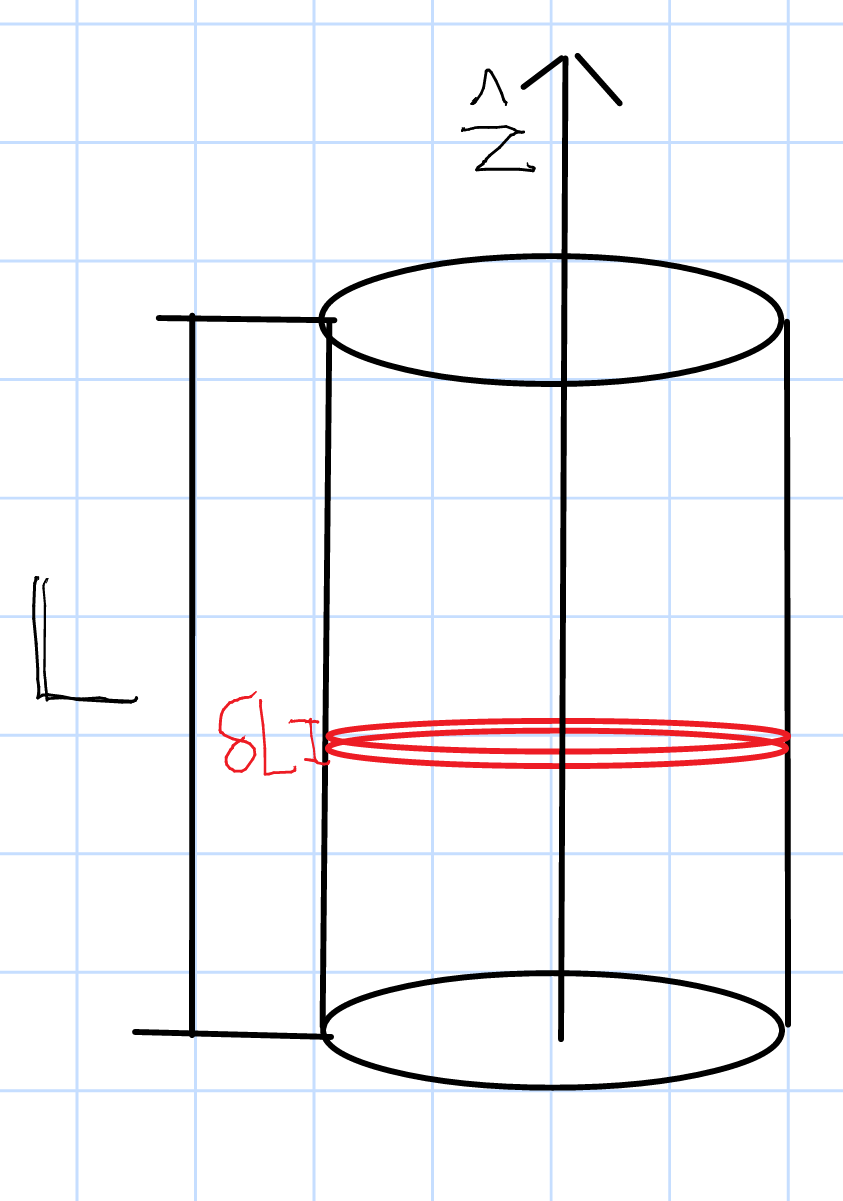
\includegraphics[width=0.3\textwidth]{cilindro.png}
\end{figure} 

Obtida então expressões matemáticas para algumas das características do helimagneto, será desenvolvido um script em Python 3 para que se faça uma visualização das mesmas. Considerando a dificuldade de se visualizar grandezas vetoriais em um cilindro, adotarei o procedimento de gerar gráficos da superfície deste, melhor ilustrado pela figura \ref{fig:recorte}

\begin{figure}
    \caption{Ilustração do "recorte" do cilindro}
    \label{fig:recorte}
    \centering
    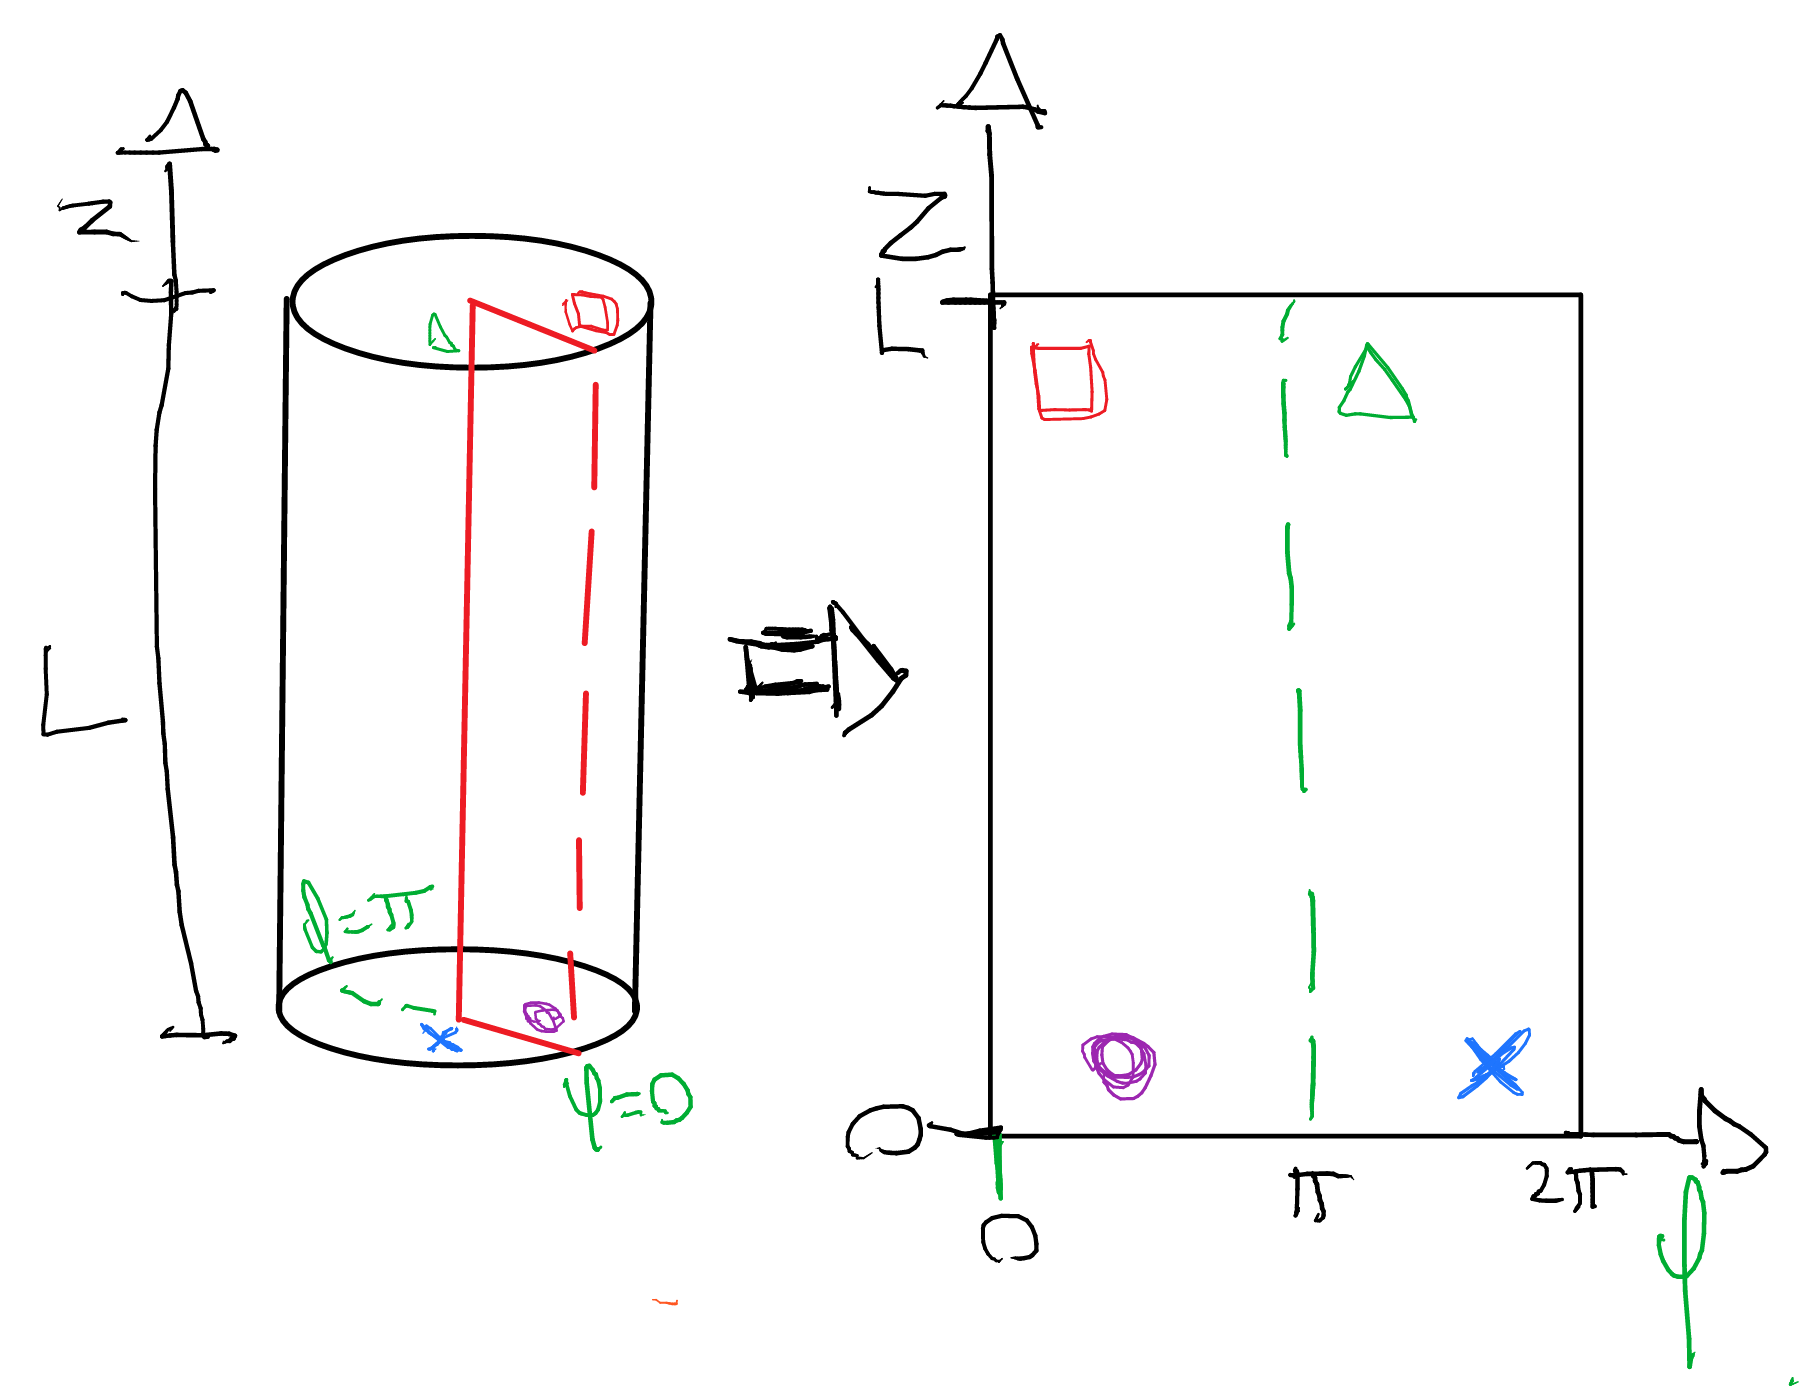
\includegraphics[width=0.4\textwidth]{recorte.png}
\end{figure}

%%%%%% %%%%%%
\section{Resultados}

%%%%%%
\subsection{Magnetização no plano xy}

Neste modelo, o vetor magnetização rotacionará no plano xy, isto é, ao longo de um plano paralelo a base do cilindro. (figura \ref{fig:magnetizacao_xy})

\begin{figure}
    \caption{Magnetização helicoidal 
    no plano xy em um cilindro}
    \label{fig:magnetizacao_xy}
    \centering
    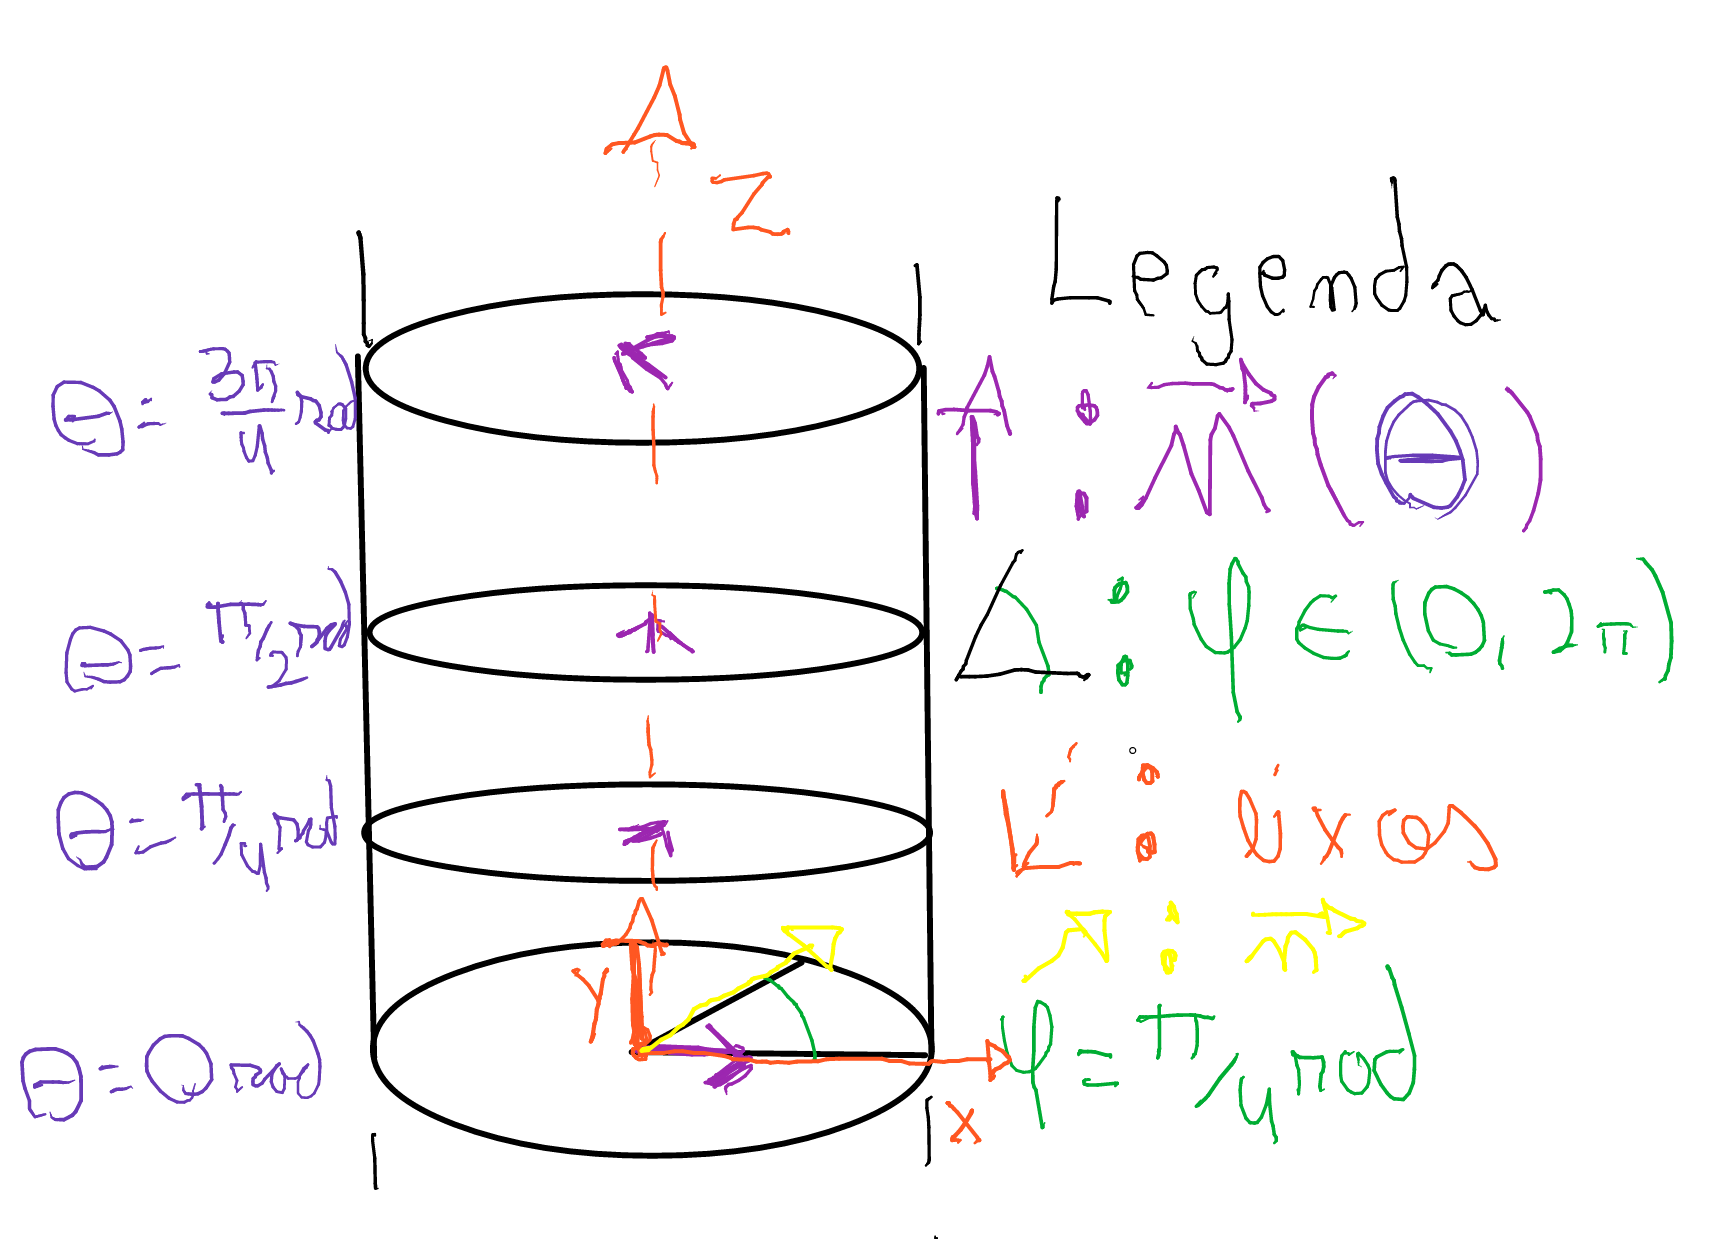
\includegraphics[width=0.4\textwidth]{magnetizacao_xy.png}
\end{figure}

Suponhamos que a magnetização no cilindro esteja orientado para $\hat{x}$ em $z=0$ e que a magnetização irá rotacionar no sentido anti-horário, então a magnetização pode ser escrita pela equação \ref{eq:M1}

\begin{equation} \label{eq:M1}
	\vec{M} = M_0 (\hat{x} \cos{\theta} + \hat{y}\sin{\theta})
\end{equation}

Faz-se também-se o postulado dado pela eq. \ref{eq:theta_z}, associando-se o período de uma revolução completa com a altura do cilindro, onde L seria a altura do cilindro. 

\begin{equation} \label{eq:theta_z}
  \theta = \frac{2 \pi z}{L}
\end{equation}

Fazendo a substituição de $\theta$ em $z$ temos que a magnetização em função somente das coordenadas é dada pela eq. \ref{eq:M1_coord}

\begin{equation} \label{eq:M1_coord}
  \vec{M} = M_0 (\hat{x} \cos{\frac{2 \pi z}{L}} + \hat{y}\sin{\frac{2 \pi z}{L}})
\end{equation}

Utilizando  a definição da corrente volumétrica ligada no caso magnetostático, teremos que esta é dada pela eq. \ref{eq:M1_volumetrico}

\begin{equation} \label{eq:M1_volumetrico}
  \vec{j_b} = \nabla \times \vec{M} = \frac{-2 \pi M_0}{L}(\hat{x}\cos{\frac{2 \pi z}{L}} + \hat{y}\sin{\frac{2 \pi z}{L}})
\end{equation}

Enquanto que a corrente superficial ligada ao longo da face lateral é dada pela eq. \ref{eq:M1_superficial}, onde o vetor normal é dado pela eq. \ref{eq:n_lat}

\begin{equation} \label{eq:M1_superficial}
  \vec{K_b} = \vec{M} \times \hat{n} = \hat{z} M_0 \sin{(\phi - \frac{2 \pi z}{L})}
\end{equation}

\begin{equation} \label{eq:n_lat}
	\hat{n} = \hat{x} \cos{\phi} + \hat{y} \sin{\phi}, \phi \in [0, 2\pi]
\end{equation}

Ao longo da face superior (sinal positivo) e inferior (sinal negativo) de um elemento de cilindro (figuras \ref{fig:cilindro}), a corrente superficial é dada pela eq. \ref{eq:M1_superficial_topo}, usando-se a eq. \ref{eq:n_topo} como vetor normal.

\begin{equation} \label{eq:M1_superficial_topo}
	\vec{K_b} = \pm M_0(-\hat{y} \cos{\theta} + \hat{x}\sin{\theta})
\end{equation}

\begin{equation} \label{eq:n_topo}
	\hat{n} = \pm \hat{z}
\end{equation}

Se fizermos a suposição de que o parâmetro de rede $\alpha$ é muito pequeno, então a corrente superficial no topo do elemento do cilindro será aproximadamente igual em magnitude e oposta em direção em relação a corrente inferior do elemento sucessivo. Tomando isso como verdadeiro, as equações \ref{eq:M1_volumetrico} e \ref{eq:M1_superficial} representam a descrição completa das correntes ligadas para o cilindro.

Uma visualização das correntes tanto volumétricas quanto as superficiais podem ser vistas na figura \ref{fig:helimagneto1}, o qual ilustra as correntes na superfície do cilindro em função de $\theta$ e do ângulo $\phi$ associado a equação \ref{eq:n_lat}. Para a figura, foram considerados $M_0 = 1$ e $L=2\pi$.

\begin{figure*}
    \caption{Magnetização no plano xy. Flechas representam correntes superficiais enquanto que as cores representam a correte volumétrica normal com a superfície}
    \label{fig:helimagneto1}
    \centering
    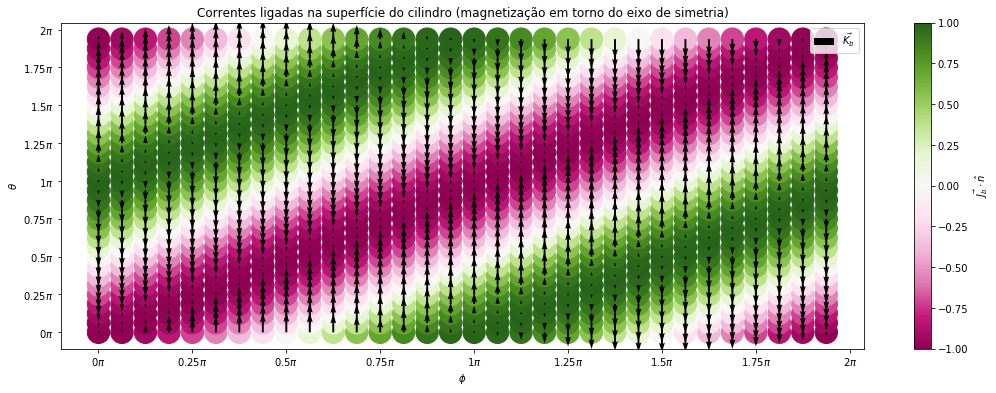
\includegraphics[width=1\textwidth]{helimagneto1.png}
\end{figure*}

É possível notar uma certa elegância neste modelo: os pontos onde o fluxo da corrente volumétrica possui direção a modo a sair do cilindro são a origem das correntes superficiais as quais estão direcionadas para os pontos onde o fluxo da corrente volumétrica possui direção a entrar dentro do cilindro. Tudo isso em um padrão helicoidal.

%%%%%%
\subsection{Magnetização no plano xz}

Um segundo exemplo com um comportamento mais complicado se trata de um vetor magnetização que oscile perpendicular em relação a base de um cilindro (fig. \ref{fig:magnetizacao_xz}).

\begin{figure}
    \caption{Magnetização helicoidal 
    no plano xz em um cilindro}
    \label{fig:magnetizacao_xz}
    \centering
    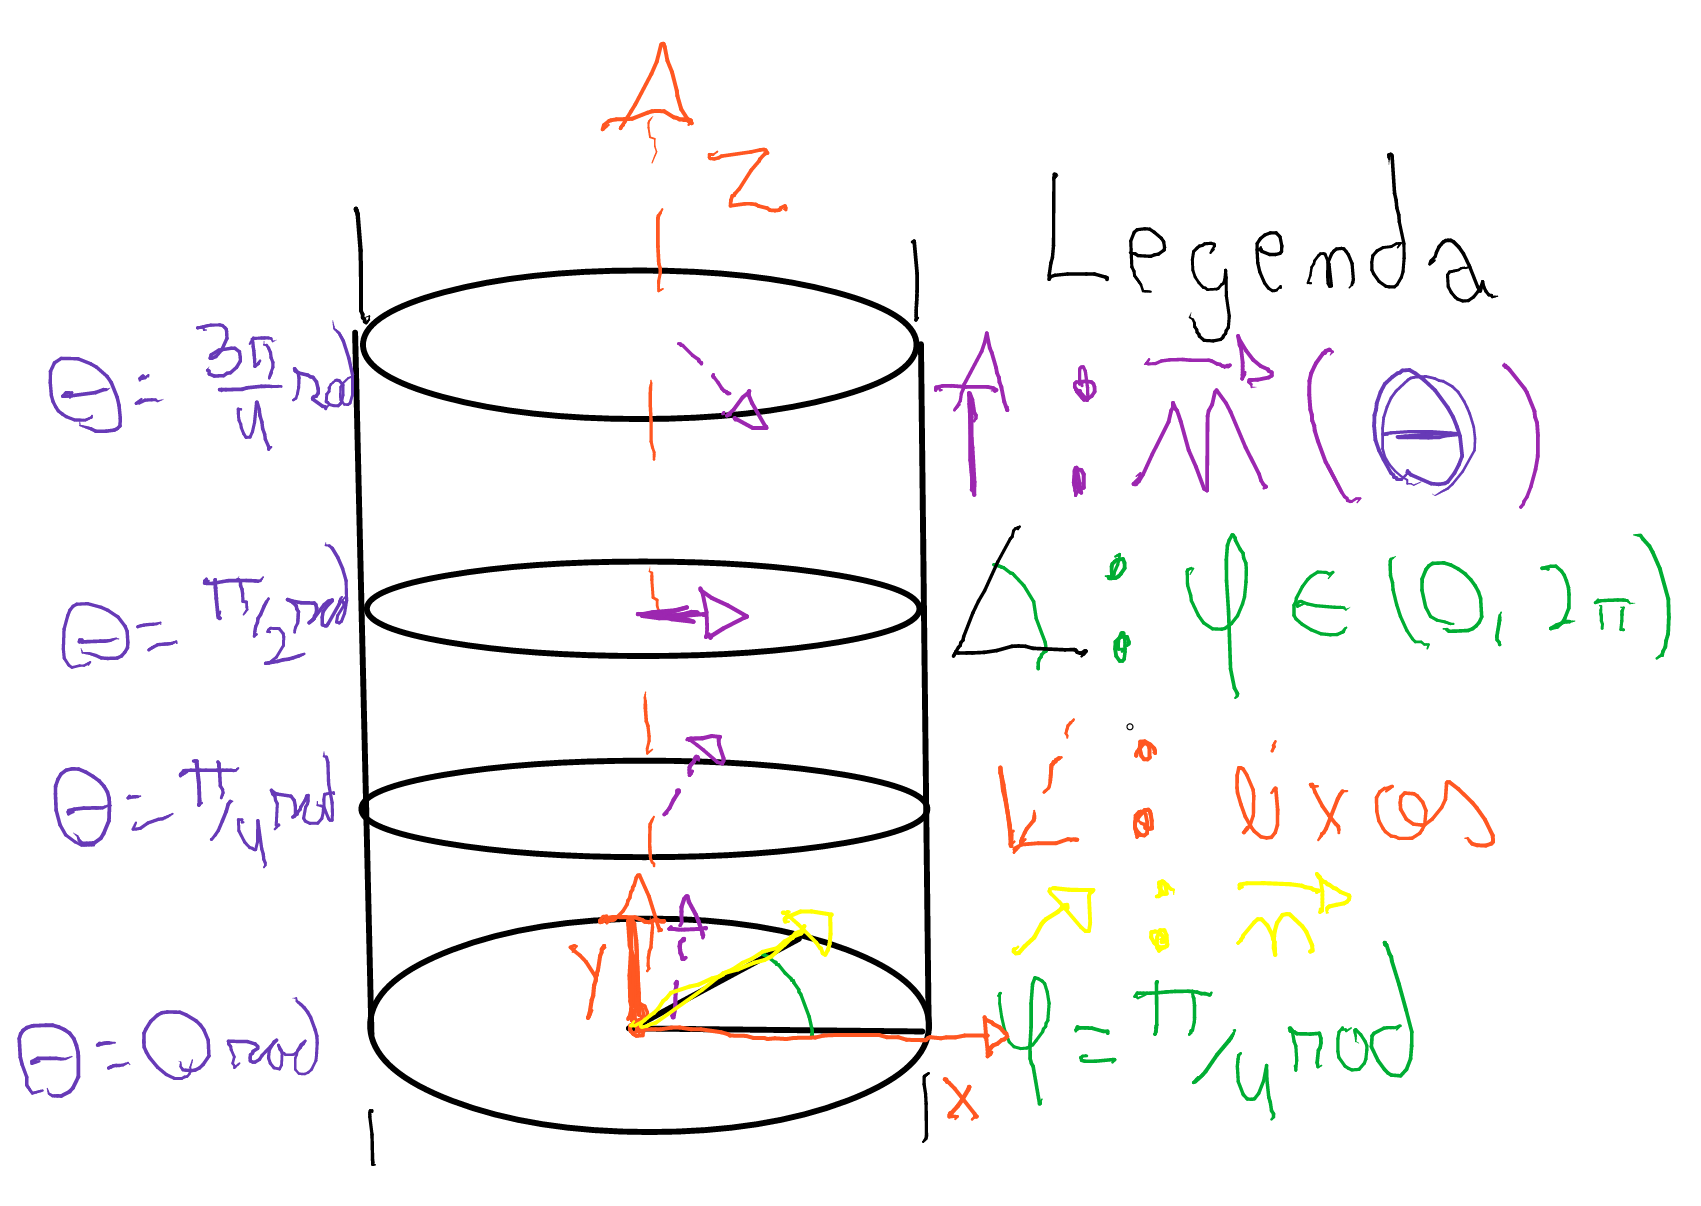
\includegraphics[width=0.4\textwidth]{magnetizacao_xz.png}
\end{figure}

É feita, para este modelo, a suposição de que o vetor magnetização é descrito pela eq. \ref{eq:M2}, que representa uma magnetização inicial orientada no eixo $\hat{z}$ rotacionando ao longo do plano xz. Adicionalmente, é feita uma suposição idêntica com o do modelo anterior de que o ângulo de rotação é proporcional a altura percorrida no cilindro (eq. \ref{eq:theta_z}), na qual implica na eq. \ref{eq:M2_theta}

\begin{equation} \label{eq:M2}
  \vec{M} = M_0 (\hat{x} \sin{\theta} + \hat{z}\cos{\theta})
\end{equation}

\begin{equation} \label{eq:M2_theta}
  \vec{M} = M_0 (\hat{x} \sin{(\frac{2 \pi z}{L})} + \hat{z}\cos{(\frac{2 \pi z}{L})})
\end{equation}

Procedendo de modo análogo com o modelo anterior, tem-se que as correntes ligadas volumétricas e superficiais são dadas pelas eq. \ref{eq:M2_volumetrica}, \ref{eq:M2_superficial} e \ref{eq:M2_superficial_topo}.

\begin{equation} \label{eq:M2_volumetrica}
  \vec{j_b} = \nabla \times \vec{M} = -\hat{y} \frac{2 \pi M_0}{L}  \sin{(\frac{2 \pi z}{L})}
\end{equation}

\begin{equation} \label{eq:M2_superficial}
\begin{split} 
  \vec{K_b}^{lateral} = \vec{M} \times \hat{n} = M_0(-&\hat{x} \cos{(\frac{2 \pi z}{L})}\sin{\phi} + \\& 
  \hat{y}\cos{(\frac{2 \pi z}{L}})\cos{\phi} + \\& 
  \hat{z} \sin{(\frac{2 \pi z}{L})} \sin{\phi} )
\end{split}
\end{equation}

\begin{equation} \label{eq:M2_superficial_topo}
	\vec{K_b}^{topo/fundo} = \pm M_0 \sin{\theta} \hat{y}
\end{equation}

Novamente, é assumido que o parâmetro de rede $\alpha$ é muito pequeno e que portanto as correntes superficiais do topo/fundo do elemento de cilindro aproximadamente se anulam mutualmente, sendo assim portanto as eqs. \ref{eq:M2_volumetrica} e \ref{eq:M2_superficial} representam a descrição completa das correntes ligadas do cilindro.

Uma forma de melhor visualizar a expressão da corrente superficial é separá-la em componentes perpendiculares e paralelos a $\hat{z}$,  nas quais se obtém as eqs. \ref{eq:M2_separated}, \ref{eq:M2_perpendicular} e \ref{eq:M2_parallel} ao considerar a eq. \ref{eq:M2_zxn}. 

\begin{equation} \label{eq:M2_zxn}
  \hat{z} \times \hat{n} = -\hat{x} sin{\phi} + \hat{y} \cos{\phi}
\end{equation}

\begin{equation} \label{eq:M2_separated}
  \vec{K_b} = M_0 (\hat{z} \times \hat{n} \cos{\theta} + \hat{z} \sin{\theta} \sin{\phi})
\end{equation}

\begin{equation} \label{eq:M2_perpendicular}
  K_{b} \bot \hat{z} = M_0 \cos{\theta}
\end{equation}

\begin{equation} \label{eq:M2_parallel}
	K_{b} \parallel \hat{z} = M_0 \sin{\theta} \sin{\phi}
\end{equation}

Utilizando as expressões acima com as suposições de $M_0=1$ e $L=2\pi \leftrightarrow z = \theta$, é possível fazer um código computacional para visualizar as correntes ligadas na superficie do cilindro, cujo resultado está na fig. \ref{fig:helimagneto2}.

\begin{figure*}
    \caption{Magnetização no plano xy. Flechas representam as correntes superficiais ligadas e as cores representam a correte volumétrica ligada normal a superfície lateral}
    \label{fig:helimagneto2}
    \centering
    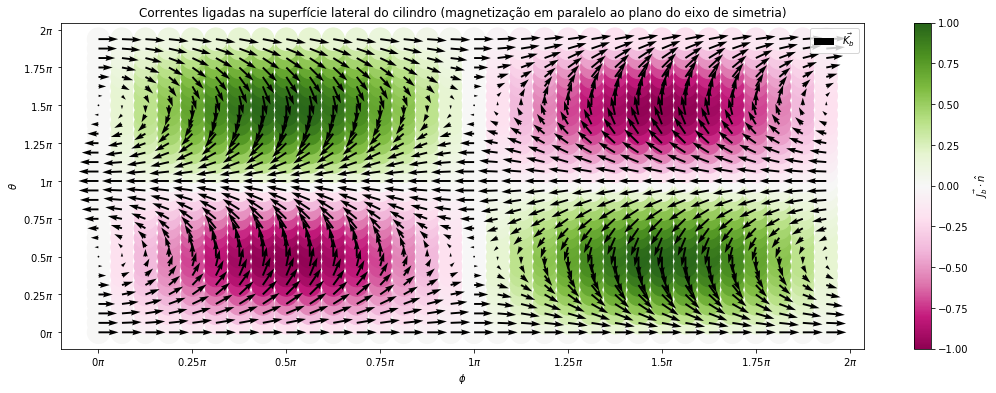
\includegraphics[width=1\textwidth]{helimagneto2.png}
\end{figure*}

É interessante notar a aparição de vórtices e anti-vórtices nas correntes superficiais neste modelo de helimagneto, e que os mesmos estão associados a pontos na qual o fluxo de corrente volumétrica normal a superficie é nulo, ou então aos pontos onde o fluxo da magnetização normal a superficie lateral é máximo/mínimo.

\section{Conclusões}

O estudo de modelos magnetostáticos como analogia ao helimagnetismo demonstrou apresentar características curiosas, como a formação espontânea de vórtices de correntes superficiais. Adicionalmente, há uma certa elegância em ver a aplicabilidade da teoria magnetostática em situações mais complexas.

Há possibilidades de extensão deste trabalho - como por exemplo fazer uma investigação acerca da influência das correntes superficiais ligadas no topo/fundo dos elementos dos cilindros, o qual não seria desprezível para um parâmetro de rede $\alpha$ que não fosse tão pequeno perto da largura do cilindro ou período da oscilação da magnetização. Outras linhas possíveis é explorar outros modelos como helimagnetos cônicos ou então buscar gerar visualizações dos campos magnéticos oriundos dos modelos aqui explorados.

%%%%%%
\begin{thebibliography}{9}

\bibitem{griffiths}
David J Griffiths; Introduction to Electrodynamics, 5ed.  2012

\bibitem{lecture_29}
A. Phillips; Structure and Properties of Functional Materials, Lecture 29
\url{http://ph.qmul.ac.uk/~anthony/spfm/29.html}

\bibitem{helimagnetism-heisenberg-model}
E. Rastelli, L. Reatto, A. Tassi; Helimagnetism in the Heisenberg Model: New Features and Old Mechanisms - 1984.

\end{thebibliography}

\onecolumn

%%%%%%
\section{Apêndice}

%%%%%%
\subsection{Código-fonte do programa}

Os códigos foram escritos em Python 3.6.3, utilizando-se das dependências numpy 1.12.1 e matplotlib 2.0.0. 

\subsubsection{Código para a magnetização no plano xy}
\lstinputlisting[basicstyle=\tiny, breaklines=true, language=Python]{xy.py}

\subsubsection{Código para a magnetização no plano xz}
\lstinputlisting[basicstyle=\tiny, breaklines=true, language=Python]{xz.py}

\subsection{Rascunho do desenvolvimento dos modelos de magnetização}

Apesar do desenvolvimento estar melhor descrito no documento deste trabalho, a forma fluída de se expressar apresenta vantagens na expressão e ilustração em relação a uma forma estruturada e padronizada. Sendo assim, colocarei nessa subseção do apêndice alguns dos rascunhos que podem servir de fonte de ilustração para o aqui descrito.

\begin{figure*}
    \caption{Desenvolvimento da magnetização no plano xy}
    \label{fig:m1}
    \centering
    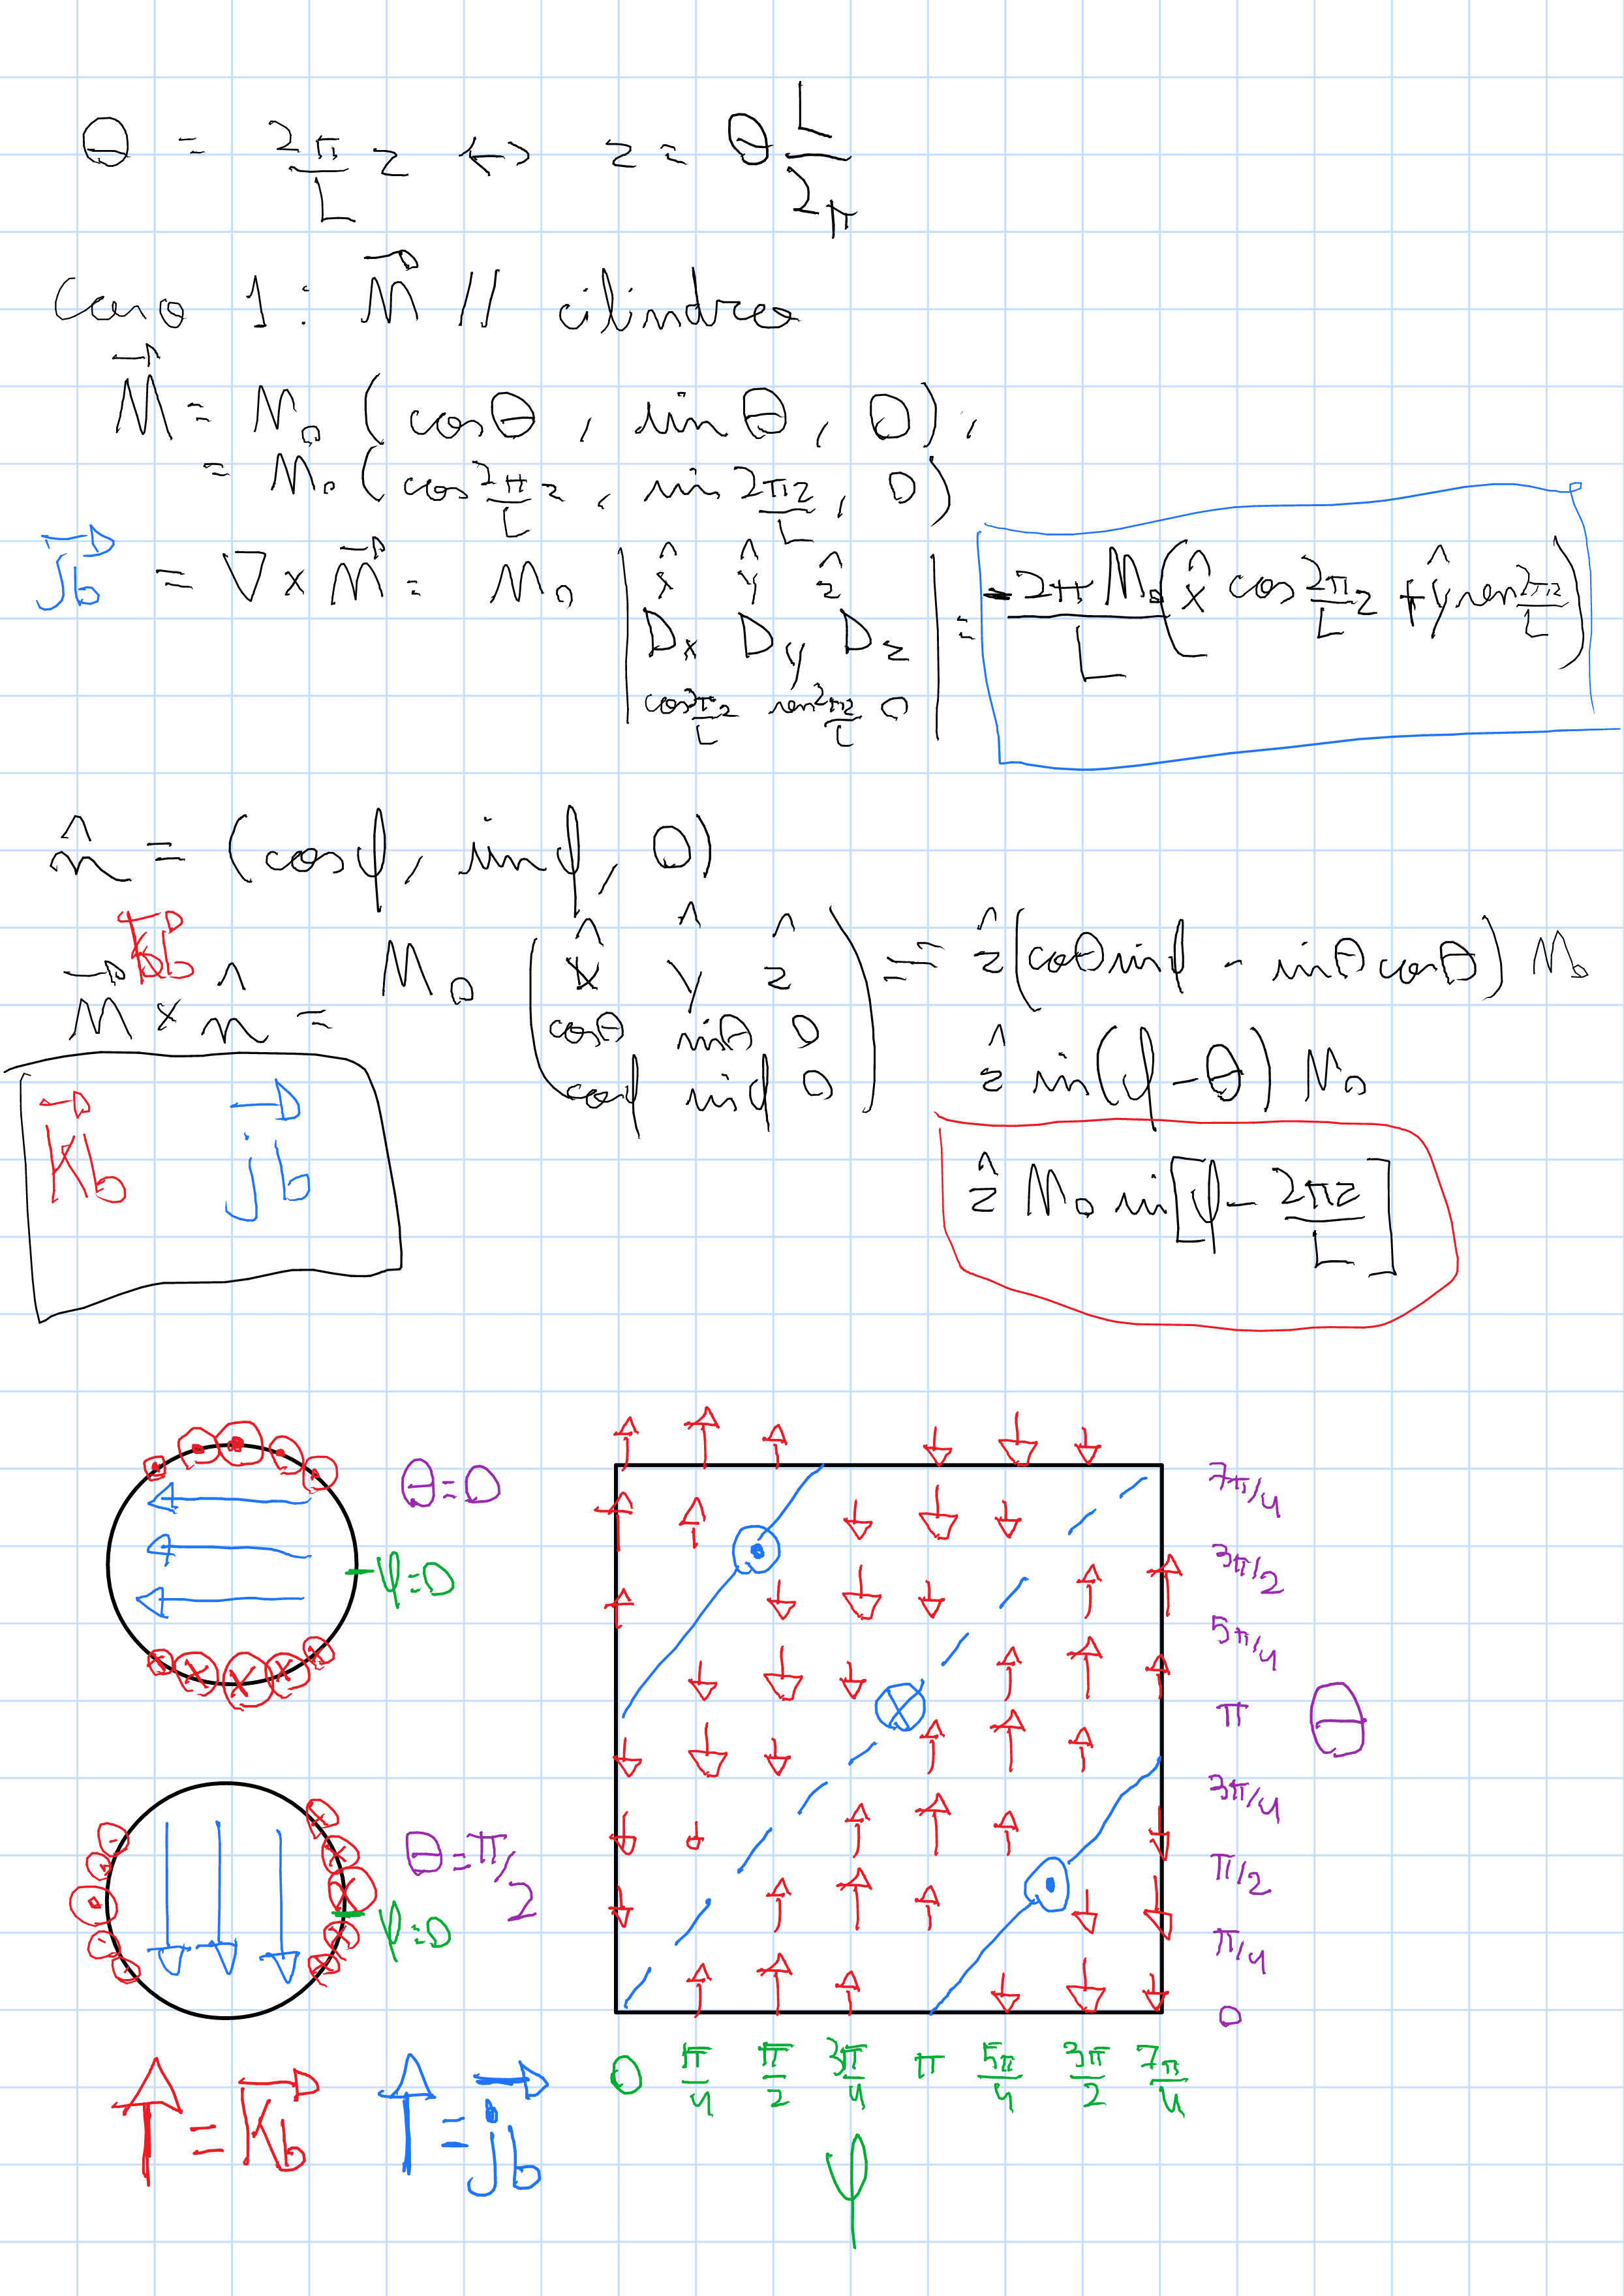
\includegraphics[width=1\textwidth]{m1.png}
\end{figure*}

\begin{figure*}
    \caption{Desenvolvimento da magnetização no plano xz}
    \label{fig:m2}
    \centering
    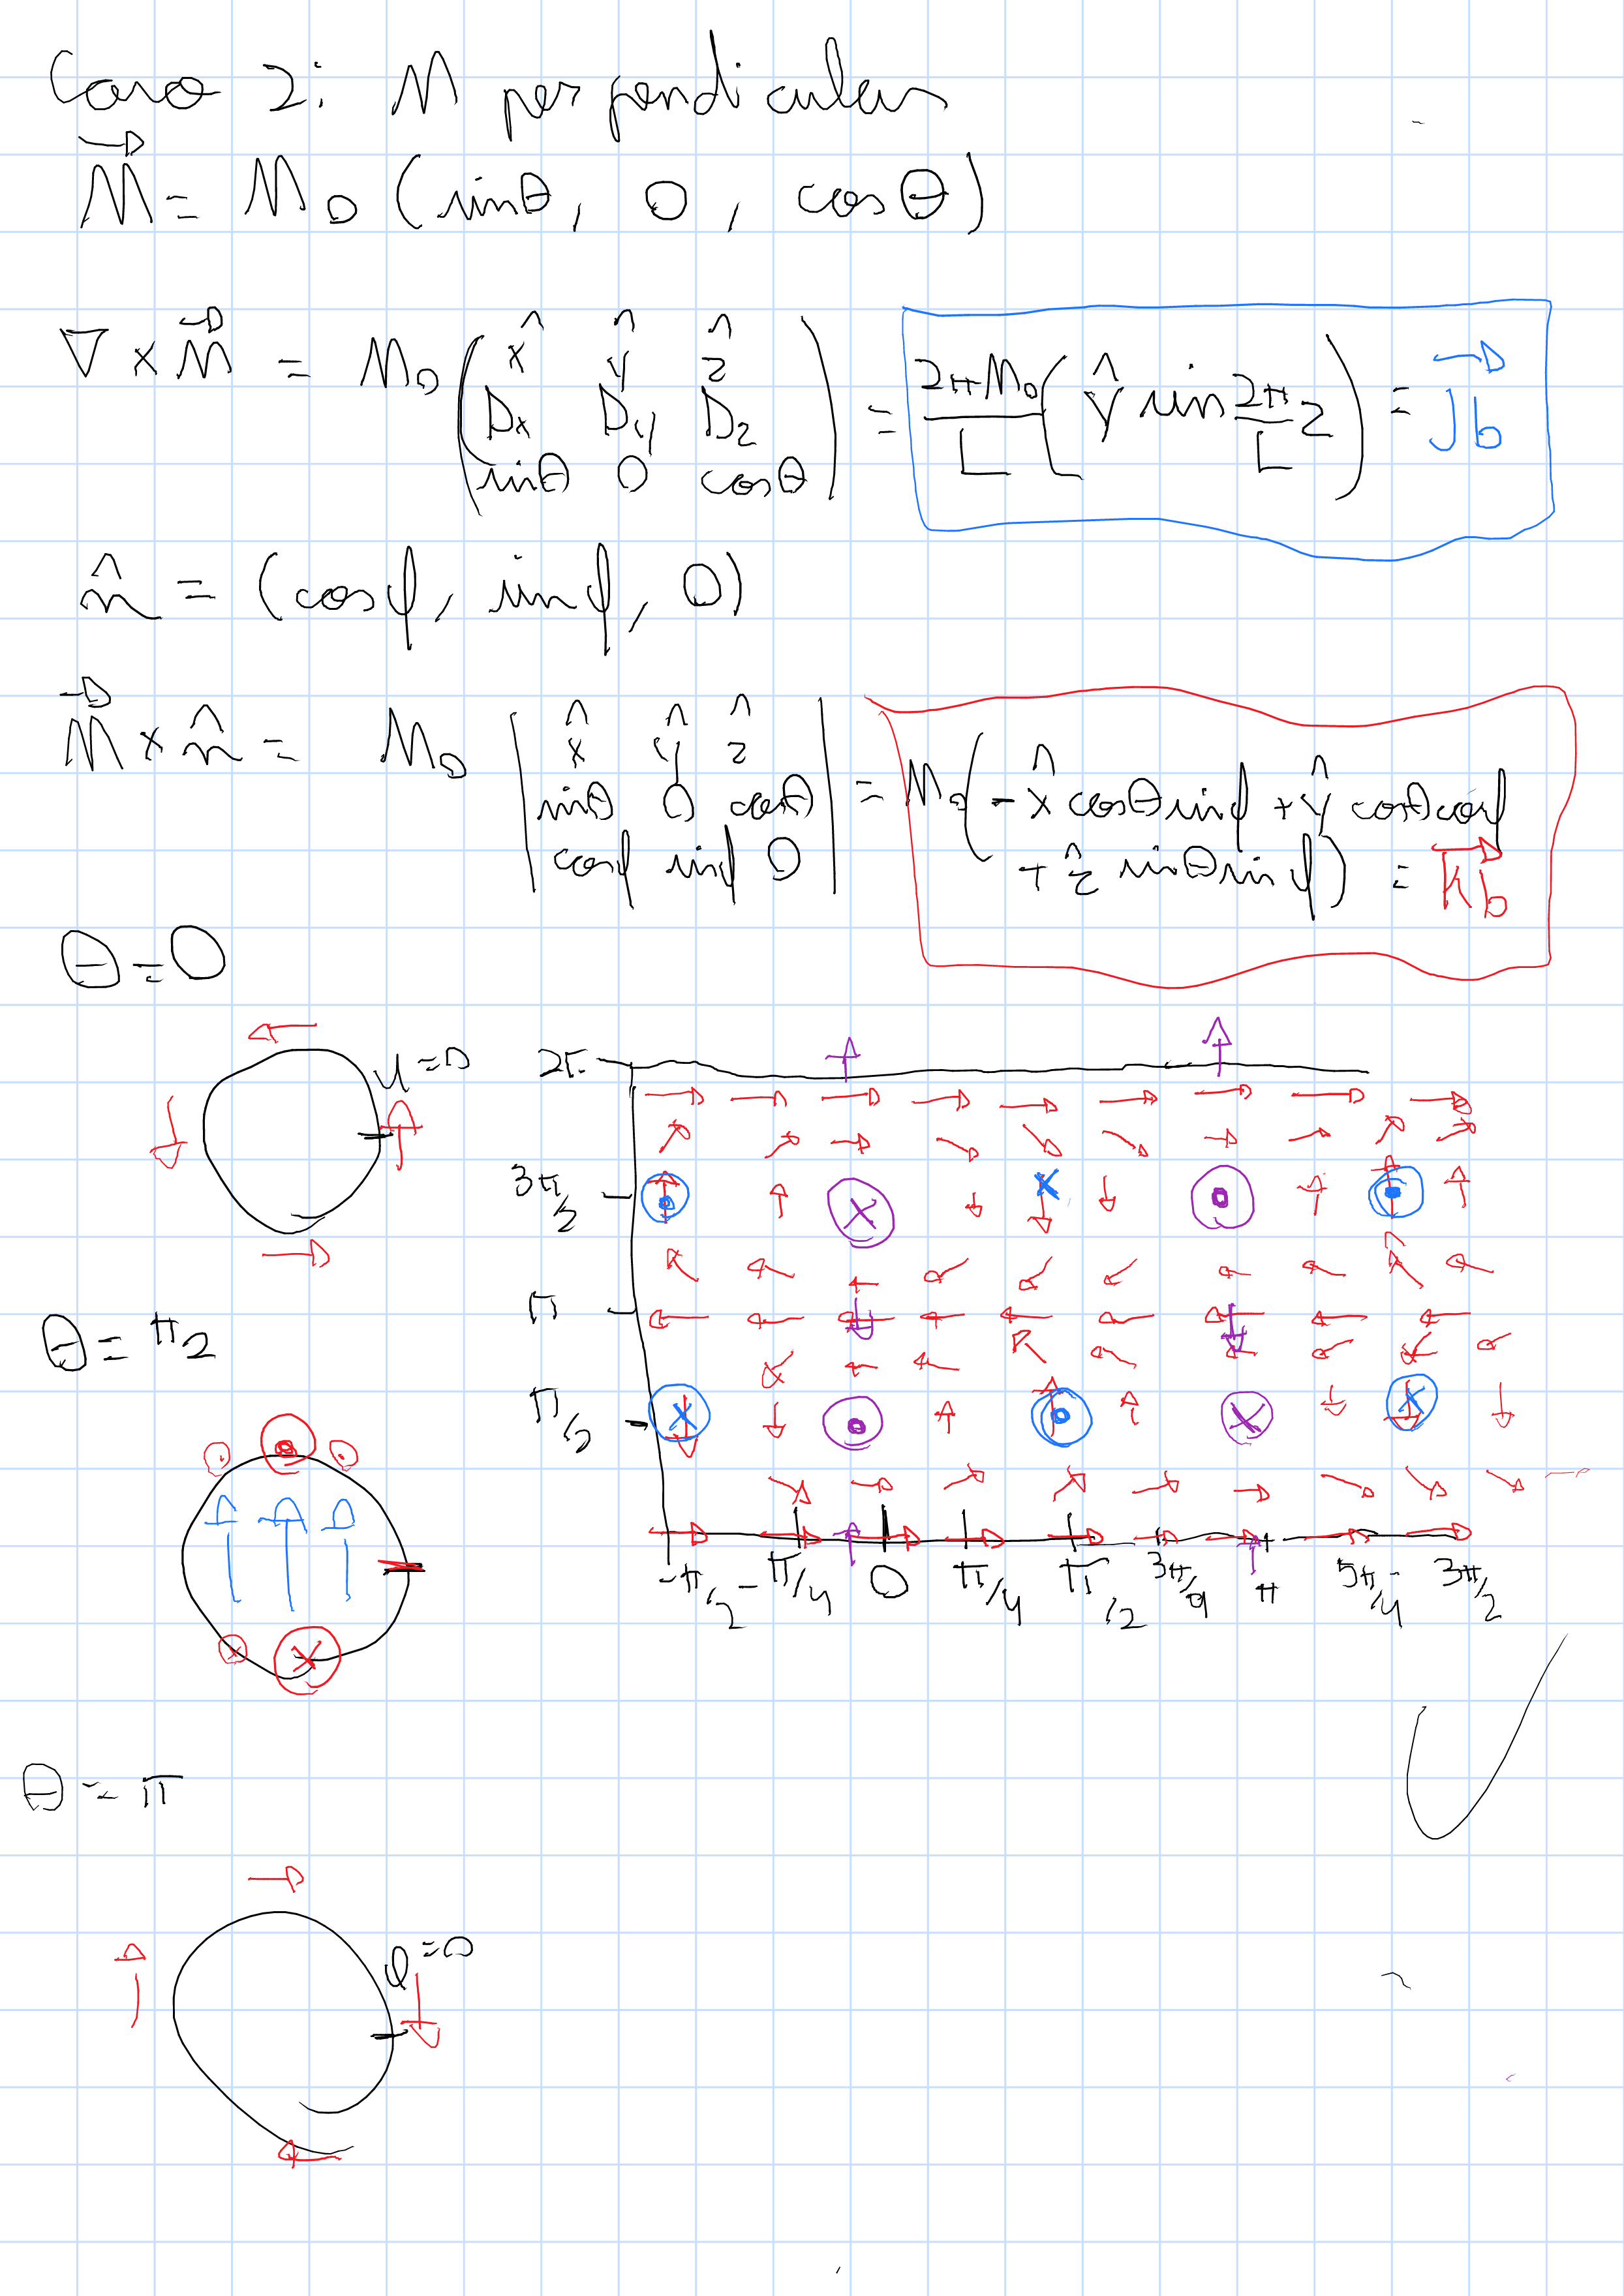
\includegraphics[width=1\textwidth]{m2.png}
\end{figure*}

\begin{figure*}
    \caption{Desenvolvimento da magnetização no plano xy (cont)}
    \label{fig:m2_cont}
    \centering
    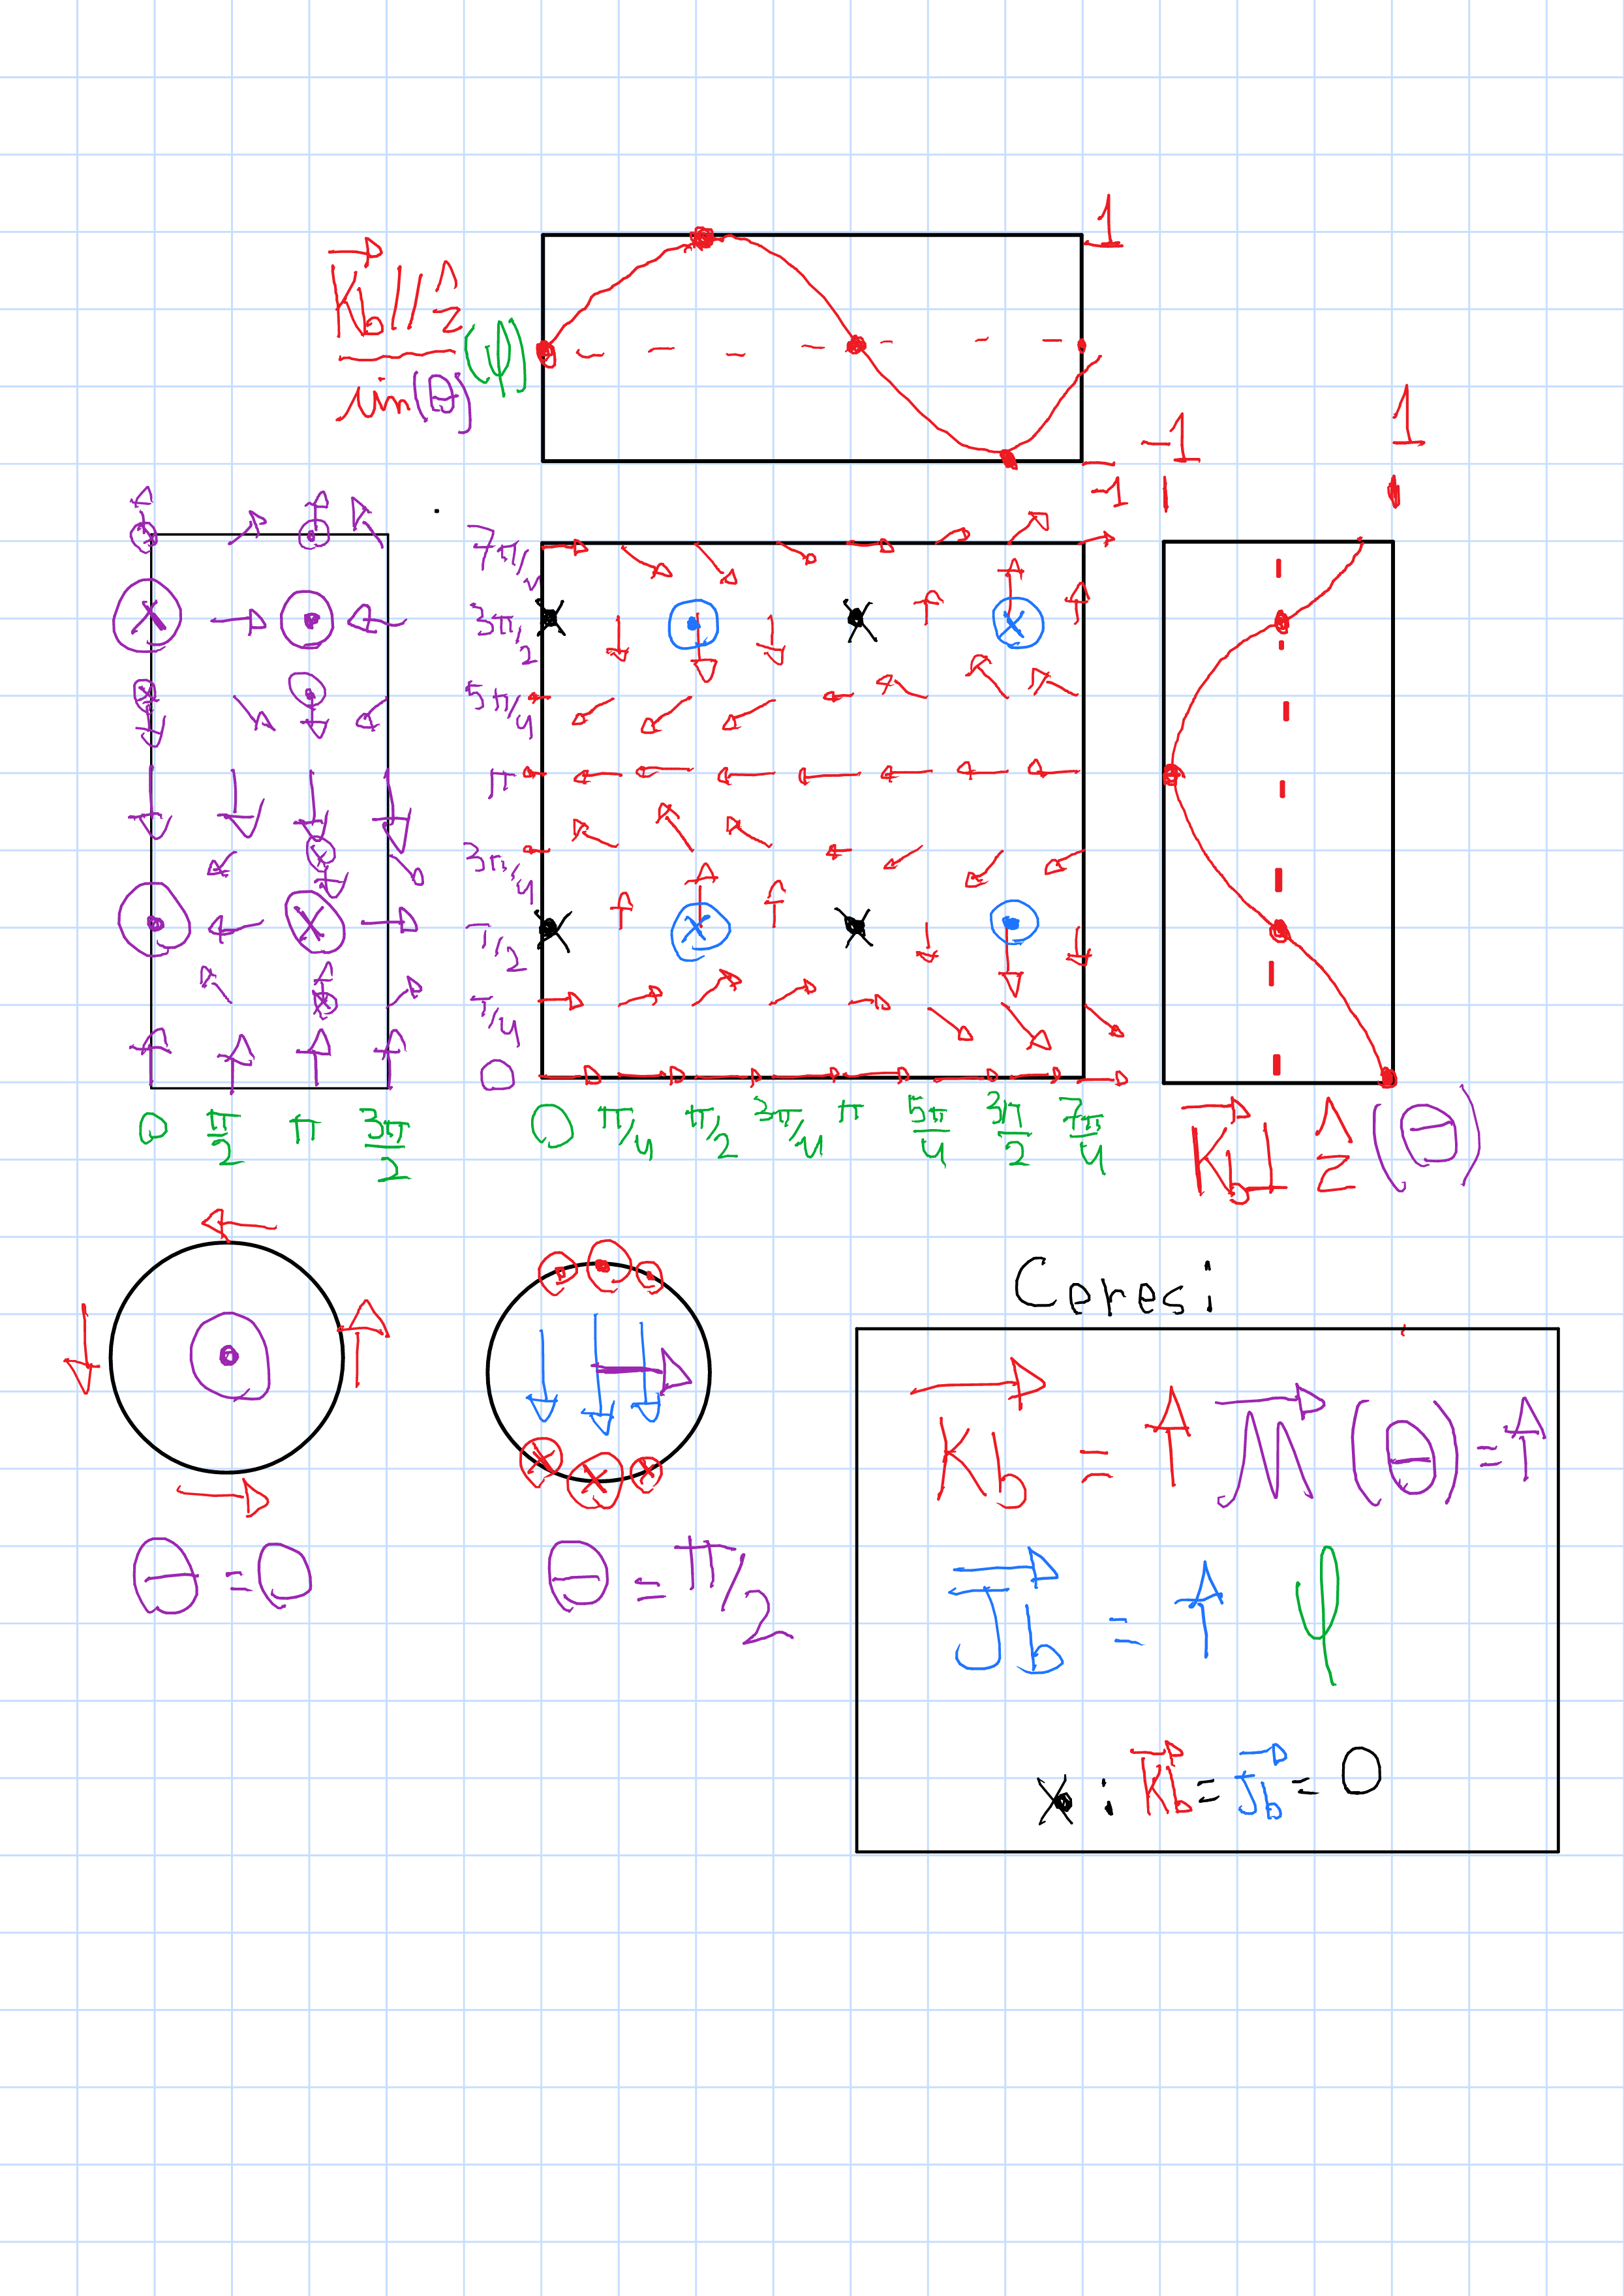
\includegraphics[width=1\textwidth]{m2_cont.png}
\end{figure*}



%%%%%%
\end{document}